\documentclass[oneside]{uniaraxatcc} % Para impressão em frente e verso, utilize twoside
\usepackage{graphicx}
\usepackage{mathtext}
\usepackage{listings}
\usepackage{amssymb}
\usepackage{color}
\usepackage{subcaption}
\usepackage[utf8]{inputenc}
\usepackage{multirow}
\usepackage{scalefnt}
\usepackage{wrapfig}
\usepackage{nomencl}
\usepackage{lipsum}

\newcommand{\uniaraxa}{\uppercase{UNIARAXÁ}}

\tipotcc{P} % P:Projeto, M: Monografia
% Nome do Curso
\curso{Sistemas de Informação}

%Qual a habilitação do curso? (Bacharel, Tecnólogo ou Licenciado(a))
\habilitacao{Bacharel}

% Autor(a) do trabalho
\autor{Carlos Gabriel \\ Guilherme Ribeiro \\ João Pedro \\ Lorayne}

% Título do Trabalho
\titulo{Bot para dicas de segurança da informação}

% Local cidade / estado
\local{Araxá}{Minas Gerais}


% Data dia / mês / ano da defesa
\date{06}{Outubro}{2022}

%Define a linha de pesquisa
% - Cultura, Desenvolvimento Humano e Gestão
% - Ambiente, Saúde e Políticas Públicas.
% - Produção, inovação e sustentabilidade.
\linhadepesquisa{Desenvolvimento de Projeto Integrador}

% Orientador [Tratamento]{Nome}{Gênero: M para Masculino e F para Feminino}
\orientador[Prof. Me]{Humberto Gustavo de Melo}{M}

% Membros da banca, podem ser definidos 2 membros de A a B (sendo que o orientador e o co-orientador já  são membros da banca)

% Primeiro membro da banca (Obrigatório)
\avaliadorA[Profa. Me.]{Nome do Membro 1}{F}

% Segundo membro da banca (Opcional)
\avaliadorB[Prof. Me.]{}{M}

% Dedicatória (Opcional)
\dedicatoria{Dedicatória não obrigatória. }

% Agradecimentos (Opcional)
\agradecimentos{\noindent\chapter*{\uppercase{Agradecimentos}}

Agradecemos ao professor Humberto pelos ensinamentos e a todos que estiveram conosco durante o semestre, nos ajudando, trocando ideias e acompanhando esta jornada. Muito obrigado.}

% Epígrafe (Opcional)
\epigrafe{\input{Partes/Epigrafe.tex}}

% Resumo (Obrigatório)
\resumo{\noindent\chapter*{\uppercase{Resumo}}

\hspace{3} Este trabalho trata-se de desenvolver um chatbot na plataforma Chatfuel, sendo implantada na rede social Facebook, o chatbot possibilita a organização e o melhoramento do atendimento a pessoas de diversos níveis de conhecimento, sendo o mesmo ágil e direto no que diz respeito de sanar as dúvidas e resolver problemas simples enfrentados pelo usuário.

\vspace{1cm}

\noindent \textbf{Palavras-chaves}:Projeto, Segurança na Internet, Projeto Integrador, Chatbot, Educação computacional.}

% Abstract (Obrigatório)
\abstract{\noindent\chapter*{\uppercase{Abstract}}

This work is about developing a chatbot on the Chatfuel platform, being implemented on the social network Facebook, the chatbot enables the organization and improvement of care to people of various levels of knowledge, being the same agile and direct with regard to solving doubts and solving simple problems faced by the user.

\vspace{1cm}

\noindent \textbf{Keywords}:Project, Internet Security, Integrator Project, Chatbot, Computer Education.}

% Siglas e Abreviações (Opcional)
\siglas{\input{Partes/Siglas.tex}}

\begin{document}
\pretextual %Indica início dos elementos pré-textuais
\maketitle %Elementos Pré-textuais
\textual %Indica início dos elementos textuais
%\pagestyle{simple}

%\chapter{\uppercase{Tema}}
%\label{tema}
%Um estudo sobre como jogos digitais podem ser usados para ensinar crianças. %Utilizado somente no Projeto de TCC
\chapter{\uppercase{Introdução}}
\label{introducao}

 Atualmente a tecnologia faz parte da vida da maioria dos brasileiros. Com o início dá pandemia, foi 
necessário adotar novos métodos de rotina para que as medidas contra a COVID-19 fossem devidamente 
obedecidos, assim, nos inserindo ainda mais no mundo digital.
Embora tenha ajudado a impulsionar a globalização, a internet também facilitou a ação de criminosos 
na rede, elevando os índices de cibercrimes. Segundo a consultoria alemã Roland Berger, o Brasil foi 
o 5° país com mais ataques cibernéticos em 2021.
Diversas informações circulam diariamente nas redes e com o aumento dos cibercrimes, saber como 
se proteger de roubos de dados e fraudes é muito importante atualmente.

Como é de conhecimento de todos, o foco e objetivo do nosso trabalho é dicas de segurança em relação a golpes e fraudes, tendo objetivos bem fixos. E diferentemente do bot criado, nosso trabalho irá utilizar de uma plataforma para se conectar a redes sociais para dar dicas e “conversar” com os usuários dando informações e dicas de como se protegerem e não cair em golpes nesse vasto mundo que é a internet, explicando tudo de forma simples.
\section{Problema e Justificativa}
\label{justificativa}

 O conhecimento básico de segurança da informação é importante dentro do
contexto atual, pois a sociedade está inserida em mundo cada vez mais digital. Contudo,
é evidente que é necessário continuamente orientar e capacitar os usuários sobre dicas
de segurança da informação.
Diversos estudos, mostram o crescimento no Brasil na perda e roubo de
informações. Em 2020, por exemplo, a empresa Karpersky através de uma pesquisa
constatou que o Brasil teve o maior número de vítimas de phishing (Valente, 2021).
Com tantas pesquisas e evidências no número do aumento de vazamento de
dados, este projeto se justifica pela possibilidade de obter ótimos resultados em benefício
da sociedade, na qual o UNIARAXÁ está inserido.
\section{Objetivos}
\label{objetivos}

%Assumindo que existe um problema a ser resolvido, apresente qual o objetivo de seu projeto de pesquisa. O que você pretende (ou pretendeu) exatamente fazer. Aqui, deve aparecer a principal ``contribuição'' de seu projeto. Qual é a principal ``coisa'' que você pretende/pretendeu fazer? Qual sua principal entrega? Não é necessário criar uma subseção para cada tipo. Pode haver uma única seção, chamada de ``objetivos'' cujo texto divida-se naturalmente em objetivo geral e objetivos específicos, deixando claro qual caso está sendo tratado em cada momento. Para diferenciar o objetivo geral dos objetivos específicos, siga as seguintes diretrizes:

\begin{itemize}

\item \textbf{Objetivo geral}: O objetivo é desenvolver uma ferramenta de conversação, via um chatbot, com processamento de linguagem natural para agilizar o atendimento. 
		
\item \textbf{Objetivos específicos}: Pesquisa bibliográfica sobre os assuntos de chatbot e helpdesk.
Realizar pesquisa dos trabalhos correlatos com este Projeto.
Identificar o público-alvo do projeto.
Definir as atividades de cada integrante do projeto.
Pesquisar sobre como construir e funcionamento de Bots e escolher uma plataforma
para desenvolvimento.
Definir os assuntos e tópicos sobre segurança da informação para aplicar no Bot.
Construção de um protótipo do Bot.
Aplicar testes no protótipo.
Analisar os resultados.
Apresentar os resultados na mostra de Extensão.
\end{itemize}

%\input{Partes/Hipotese.tex}
%\input{Partes/Limitacoes.tex}
%\input{Partes/Estrutura.tex}
\chapter{\uppercase{Referencial Teórico}}
\label{referencial}

\section{O que é um Bot?}\\
Bot é um programa de software que executa tarefas automatizadas, autônomas, repetitivas e pré-definidas. Os bots normalmente imitam ou substituem o comportamento do usuário humano. Por serem automatizados, operam muito mais rápido do que os humanos.
 
\section{Como é o funcionamento de um Bot?}\\
Os Bots funcionam como programas de computador que, através da inteligência artificial interagem, analisa e tenta copiar o comportamento humano e também simula a forma de pensar do ser humano tentando soar o mais natural possível.
Eles operam através de uma rede, e são basicamente feitos a partir de conjuntos de algoritmos que os ajudam a realizar as suas tarefas.

\section{Ferramentas de mercado sobre bots}\\
Chatbox é considerada uma das melhores ferramentas de mercado de acordo com várias pesquisas mostrando que 80\% das empresas participantes planejavam construir um chatbox para a sua empresa. No Brasil só vem crescendo ao longo dos anos e mostra o uso o uso do chatbox em diversas frentes, tanto para SAC, como na capacitação ativas de novos clientes, e até mesmo atuando no fechamento de vendas. 
As ferramentas mais usadas são: 
•	- Zenvia;\\
•	- ManyChat;\\
•	- Botsify;\\
•	- Chatfuel;\\
•	- MobileMonkey;\\
•	- Bluelab;\\
•	- Blip. 
%\input{Partes/Metodologia.tex}
%\input{Partes/Desenvolvimento.tex}
\chapter{\uppercase{Trabalhos Relacionados}}
\label{TrabalhosRelacionados}

Como é de conhecimento de todos, o foco e objetivo do nosso trabalho é dicas de segurança em relação a golpes e fraudes, tendo objetivos bem fixos. E diferentemente do bot criado, nosso trabalho irá utilizar de uma plataforma para se conectar a redes sociais para dar dicas e “conversar” com os usuários dando informações e dicas de como se protegerem e não cair em golpes nesse vasto mundo que é a internet, explicando tudo de forma simples.
\chapter{Plano de Teste}
\label{Plano de Teste}

O plano de testes:

Para deixar o bot mais preciso e confiável, faremos alguns testes com ele.:
Faremos um teste para conferir se o bot está liderando/dominando a conversa, para que o usuário não desvie do assunto principal. O ideal é que o bot tenha uma conversa fluida com o usuário. 
Testaremos também o vocabulário (Teste de Domínio). É preciso que o bot tenha um vocabulário extenso, incluindo gírias , dialetos e possíveis formas de falar a mesma frase. 

Faremos testes com grupos de pessoas internas e externas utilizando o plano de testes descrito acima. 
\begin{itemize}

\item \textbf {Primeiro:} Teste manual, entre nós mesmos. 

\item \textbf {Segundo:} será feito entre os grupos da sala. Será testado a eficiência do bot quanto ao domínio e a liderança na conversa. 

\item \textbf {Terceiro teste:} Este será feito com pessoas externas. Nosso critério de escolha é dar maior atenção para o nosso público alvo. Faremos teste com pessoas da família que tem menos conhecimento sobre o mundo virtual/tecnologia e com pessoas da família que tenha um pouco mais de conhecimento. Este teste será feito entorno de 10 à 15 pessoas.
\end{itemize}
Como o bot é aberto para todos, faremos também com pessoas que tem mais conhecimento na área, podendo ser pessoas de outros períodos ou até mesmo com mais pessoas da nossa sala. Este teste será feito entre 5 à 10 pessoas.

Como vão saber quando o bot não soube responder? 

Acompanharemos pela ferramenta toda a conversação de testes. No Chatfuel, é possível ver mensagens enviadas pelo usuário que ainda não foram automatizadas. As mensagens que tem ligação direta com o assunto, serão automatizadas após e durante a fase de testes. 

Onde nosso pode ser encontrado projeto? 

A versão final do projeto será disponibilizada no Facebook. Escolhemos o Facebook por  ser uma  plataforma mais acessível, visto  que o projeto é voltado para um público com pouco conhecimento do mundo virtual. As pessoas poderão se comunicar com o bot pelo Facebook Messenger.

\section{Plataforma Utilizada}
\label{Plataforma Utilizada}
    Utilizamos a plataforma "Facebook" para hospedar nosso bot, ela oferece diversidade de respostas e a possibilidade de implementação através da indução ao erro, o serviço do mesmo é gratuito.\\
\begin{figure}[h]
\centering
\captionsetup[subfigure]{labelformat=empty}
\caption{``Bot Anna''}
\begin{subfigure}{.5\textwidth}
\centering
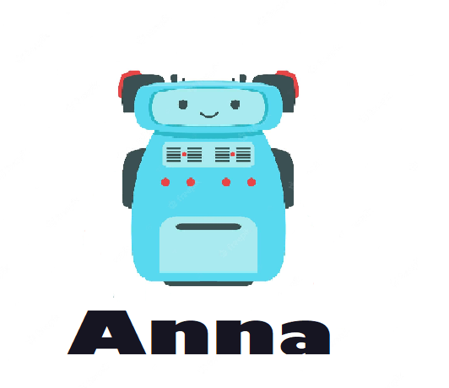
\includegraphics[width=8cm,height=6cm]{Partes/Imagens/Anna.png}
\caption{Bot criado pelo grupo (2022).}
\end{subfigure}%
\end{figure}

\section{Gráficos de confiabilidade do bot}
\label{Gráficos de confiabilidade do bot}
\begin{figure}[h]
\flushleft
\captionsetup[subfigure]{labelformat=empty}
\caption{``Acerto do perguntas de um Iniciante''}
\begin{subfigure}{.5\textwidth}
\centering
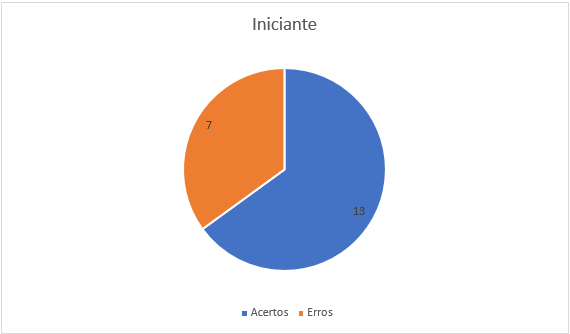
\includegraphics[width=16cm,height=8cm]{Partes/Imagens/Iniciante.png}
\end{subfigure}%
\end{figure}

\begin{figure}[h]
\flushleft
\captionsetup[subfigure]{labelformat=empty}
\caption{``Acerto do perguntas de um Avançado''}
\begin{subfigure}{.5\textwidth}
\centering
\includegraphics[width=16cm,height=8cm]{Partes/Imagens/Avançado.png}
\end{subfigure}%
\end{figure}
\chapter{\uppercase{Considerações finais}}
\label{conclusao}

No começo da disciplina quando nos foi posto a realização de um desenvolvimento de um chatbot para auxiliar as pessoas a sanar dúvidas sobre segurança na internet. Após a proposta, foi necessário fazer várias pesquisas sobre funcionamento de IAs, de BOTs e como são feitos, além de fazer pesquisas para saber da população quais são suas maiores dúvidas para sanar as mesmas e auxiliar cada vez mais as pessoas, de forma gratuita e de fácil acesso.
 
 O desenvolvimento do bot educativo ``Anna" levou em sua totalidade, quase 5 meses, foi e está sendo uma grande experiênca enriquecedora.
 
 Com as informações passadas ao longo da apresentação do Projeto Integrador, é conclusivo que os objetivos apresentados pelo P.O foram alcançados, porém é possível implementar o bot continuamente, melhorando-o.
 
  \section{Trabalhos Futuros}
  
  Este chatbot foi testado em sala, com pessoas fora de sala também, a capacidade de crescimento do bot é de certa forma conhecido, sua versão grátis é possível fazer até 50 interações. A Eficácia e confiabilidade estão diretamente ligadas ao 

%\input{Partes/Etapas.tex} %Utilizado somente no Projeto de TCC
%\input{Partes/Cronograma.tex} %Utilizado somente no Projeto de TCC

\postextual %Indica início dos elementos pós-textuais	

\bibliography{Referencias}

\begin{anexosenv}
% Imprime uma página indicando o início dos anexos
	%\partanexos

%(opcional)
\label{Referências}\\https://blog.hdstore.com.br/tipos-ataques-ciberneticos/\\
https://techtoday.lenovo.com/br/pt/solutions/smb/5-falhas-de-seguranca-digital\\
https://www.ifsudestemg.edu.br/acessoainformacao/protecao-de-dados-pessoais-no-if-sudeste-mg/dicas\\
https://blog.ecoit.com.br/cartilha-de-seguranca-da-informacao/amp/\\
https://www.kaspersky.com.br/resource-center/definitions/what-are-bots\\
https://br.norton.com/internetsecurity-how-to-how-to-recognize-and-protect-yourself-from-cybercrime.html\\
https://leadster.com.br/blog/melhores-chatbots/\\ 
\end{anexosenv}

%(opcional)
%\input{Partes/Apendice.tex} 
\end{document}
